\documentclass{beamer}
\usetheme{}
\usecolortheme{dolphin}           
\useinnertheme{circles}
\setbeamertemplate{itemize items}[default]
\setbeamertemplate{enumerate items}[default]
\usepackage[T1]{fontenc}
\usepackage[utf8]{inputenc}
\usepackage{lmodern}
\usepackage{amsmath}
\usepackage{booktabs} 
\usepackage{graphicx}        
\usepackage{array}
\usepackage{color}
\usepackage{textcomp}
\usepackage{epstopdf}                     % For EPS figures
\makeatletter
\def\zapcolorreset{\let\reset@color\relax\ignorespaces}
\def\colorrows#1{\noalign{\aftergroup\zapcolorreset#1}\ignorespaces}
\makeatother
\graphicspath{{/home/swl/Dropbox/ucd/international_trade/tex/}} 
\setbeamertemplate{navigation symbols}{}

%--------------------------------------
%%%% DETAILS TITLE PAGE %%%%
%--------------------------------------
\title{Ricardian model}
\author{School of Economics, University College Dublin}
\date{Autumn 2017}
\begin{document}
%--------------------------------------
%%%% TITLE SLIDE %%%%
%--------------------------------------
\begin{frame}
\titlepage  
\end{frame}


%--------------------------------------
\begin{frame}
  In 2015 Ireland imported
  \begin{itemize}
    \item Bananas from Belize (7.89M USD)
    \item Soybean oilcake from Argentina (116M USD)
    \item Petroleum from Saudi Arabia (17.8M USD)
    \item Cars from Germany (695M USD)
    \item Aircrafts from the USA (2.57B)
  \end{itemize}
\end{frame}
%--------------------------------------

%--------------------------------------
\begin{frame}
  In 2015 Ireland exported
  \begin{itemize}
    \item Medicaments (24.2B USD)
    \item Heterocyclic compounds (17.3B USD)
    \item Human or animal blood (11.7B USD)
    \item Malt extract (2.1B USD)
  \end{itemize}
\end{frame}
%--------------------------------------

%--------------------------------------
\begin{frame}
  Countries trade because of
  \begin{enumerate}
    \item Proximity to each other
    \item Cross-country differences
    \begin{itemize}
      \item Resource availability/factors of production
    \end{itemize}
    \item Economies of scale and product differentiation
    \begin{itemize}
      \item Produce efficiently a limited amount of goods
    \end{itemize}
  \end{enumerate}
\end{frame}
%--------------------------------------

%--------------------------------------
\begin{frame}
  David Ricardo thought that
  \begin{enumerate}
    \item Countries trade due to technological differences
    \item Countries can always gain from trade
    \begin{itemize}
      \item Even a country that is better at everything
    \end{itemize}
  \end{enumerate}
\end{frame}
%--------------------------------------

%--------------------------------------
\begin{frame}
  Note that Ricardo lived in a time of mercantilism which has a strong focus on a positive trade balance
  \begin{itemize}
    \item Exports good, imports bad
  \end{itemize}
  \medskip
  As a result, mercantilism is in favour of high tariffs in order to reduce imports
  \begin{itemize}
    \item e.g. the corn laws in the UK at the time of Ricardo (1815-1846)
  \end{itemize}
  \medskip
  In contrast, Ricardo showed that free trade could benefit all trade partners
\end{frame}
%--------------------------------------

%--------------------------------------
\begin{frame}
\begin{table}{Quantity produced by labour force}
  \begin{tabular}{lcc}
    ~ & Cloth (m) & Wine (l) \\
    \hline \\[-1.8ex]\\	
    Portugal  & 20  & 300\\
    England & 10  & 100\\    
  \end{tabular}
\end{table}
\end{frame}
%--------------------------------------

%--------------------------------------
\begin{frame}
  Although Portugal has \textbf{absolute} advantage in producing both goods, yet it can still benefit from trade
  \medskip
    \begin{enumerate}
      \item England should specialise in producing cloth: has a \textbf{comparative} advantage
      \item Portugal should specialise in producing wine    
    \end{enumerate}
\end{frame}
%--------------------------------------

%--------------------------------------
\begin{frame}
  Under specialisation Portugal could trade 300L of wine against 30m of cloth
  \begin{align*}
    300 \cdotp \frac{10}{100}    
  \end{align*}
  \begin{itemize}
    \item Would give up 20m of cloth to produce additional 300L of wine
  \end{itemize}
  \medskip
  England could trade 10m of cloth against 150L of wine
  \begin{align*}
    10 \cdotp \frac{300}{20}
  \end{align*}
  \begin{itemize}
    \item Give up 100L of wine for 10m of cloth
  \end{itemize}
\end{frame}
%--------------------------------------

%--------------------------------------
\begin{frame}
  \begin{itemize}
    \item England has comparative advantage in producing cloth
    \item Portugal has comparative advantage in producing wine    
  \end{itemize}
  Both countries gain by specialising and trading.
\end{frame}
%--------------------------------------

%--------------------------------------
\begin{frame}
  Main idea of the Ricardian model is that
  \medskip
  \begin{itemize}
    \item Trade happens due to technological differences or labour productivity
    \item Countries will be benefit by specialising
  \end{itemize}
    \medskip   
    The model therefore predicts that under free trade countries will specialise.
    \begin{itemize}
     \item Free trade will benefit all participants, relative to autarky, even if some countries are terrible at everything. 
    \end{itemize}    
\end{frame}
%--------------------------------------

%--------------------------------------
\begin{frame}{Comparative advantage Italy}
  \begin{figure}
    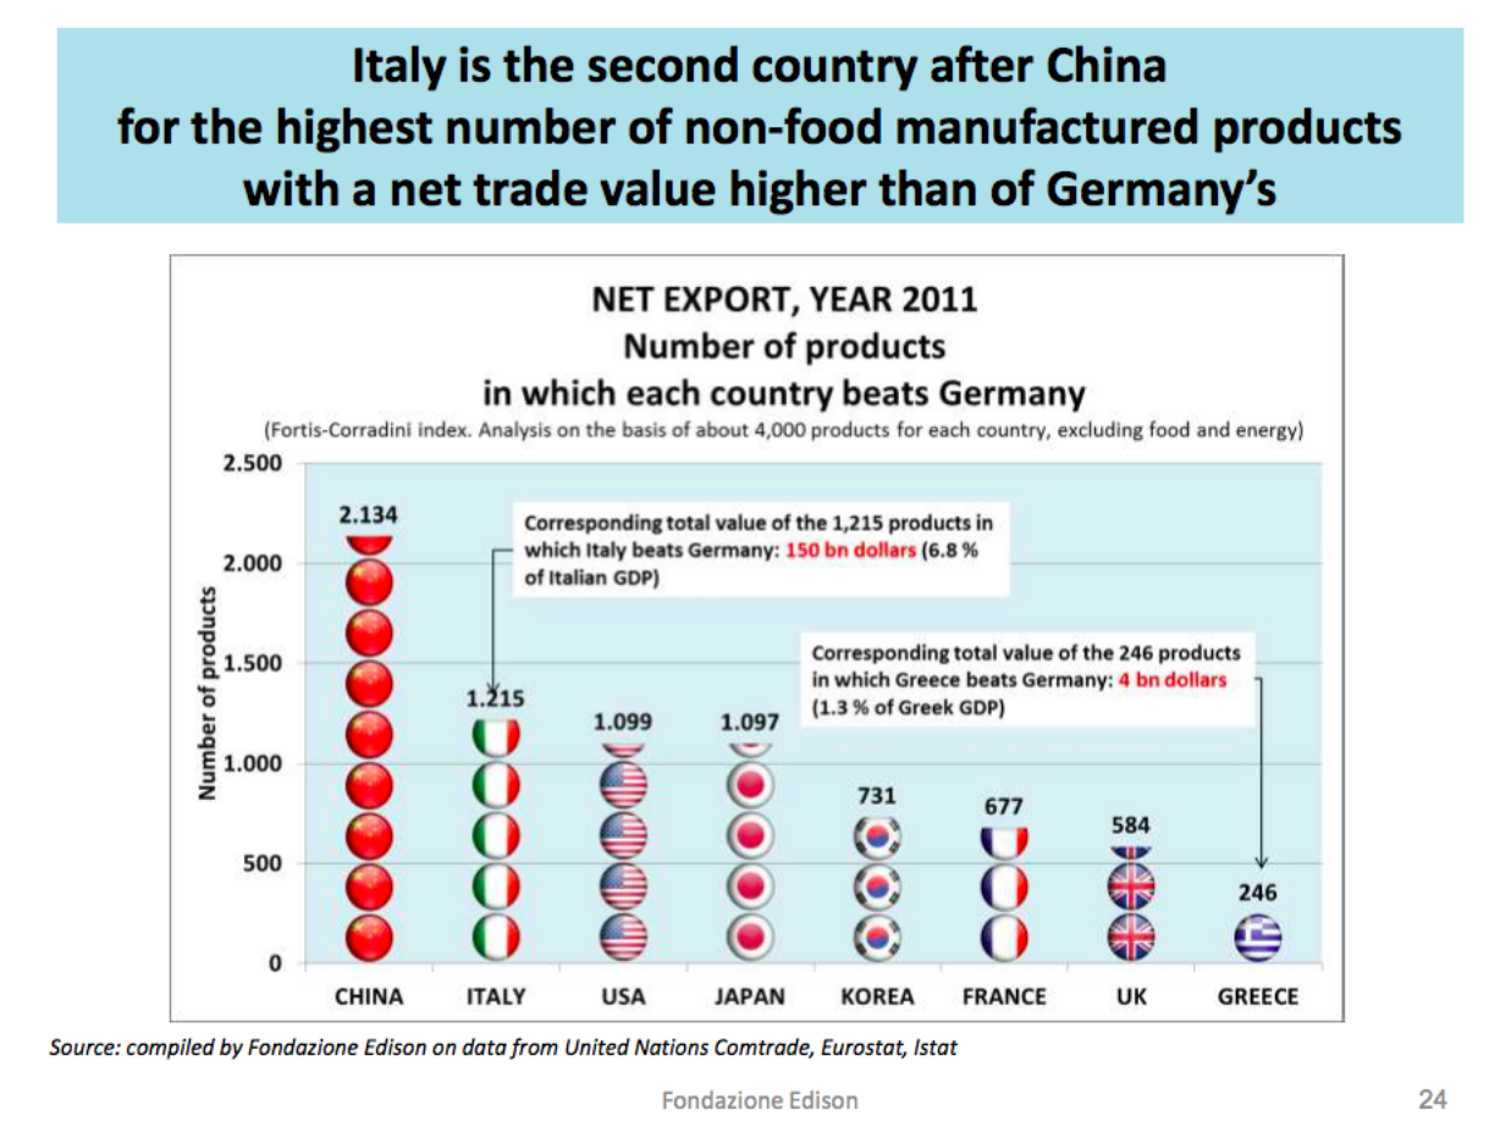
\includegraphics[scale=.8]{italy}
  \end{figure}  
\end{frame}
%--------------------------------------

%--------------------------------------
\begin{frame}
  Let's set up the formal model, in its most basic form there are
  \medskip
  \begin{itemize}
    \item 2 countries: $Home, Foreign$
    \item 2 goods: $X, Y$
    \item 1 production factor: labour $L$
  \end{itemize}
\end{frame}
%--------------------------------------

%--------------------------------------
\begin{frame}
  The supply assumption is that labour $L$ is mobile across sectors and is competitive
  \begin{itemize}
    \item Workers move to sector with higher wages
  \end{itemize}
  \medskip
  Moreover the labour supply is constant and cannot move between countries
  \begin{itemize}
    \item Production with constant returns to scale     
  \end{itemize}      
\end{frame}
%--------------------------------------

%--------------------------------------
\begin{frame}
  For demand the model assumes that consumers consume goods to maximise utility and consumption is constrained by labour income
  Demand assumptions include
  \medskip
  \begin{itemize}
    \item Price increase in one good leads to substitution with other good    
  \end{itemize}
  \medskip
  Importantly under free trade the consumed goods can be produced anywhere.
\end{frame}
%--------------------------------------

%--------------------------------------
\begin{frame}
  $Home$ has $L$ hours of labour\\
  \begin{itemize}
    \item One unit of $x$ takes $a_x$ hours
    \item One unit of $y$ takes $a_y$ hours
  \end{itemize}
  \medskip
  $Foreign$ has $L^*$ hours of labour
  \begin{itemize}
    \item One unit of $x$ takes $a_x^*$ hours
    \item One unit of $y$ takes $a_y^*$ hours
  \end{itemize}
\end{frame}
%--------------------------------------

%--------------------------------------
\begin{frame}
  Production is constrained by labour supply $L$ and the production possibilities frontier (PPF) is given by
  \begin{align*}
    L=a_xX+a_yY\\
    L^*=a_x^*X+a_y^*Y
  \end{align*}
\end{frame}
%--------------------------------------

%--------------------------------------
\begin{frame}{Example of PPF}
  \begin{figure}
    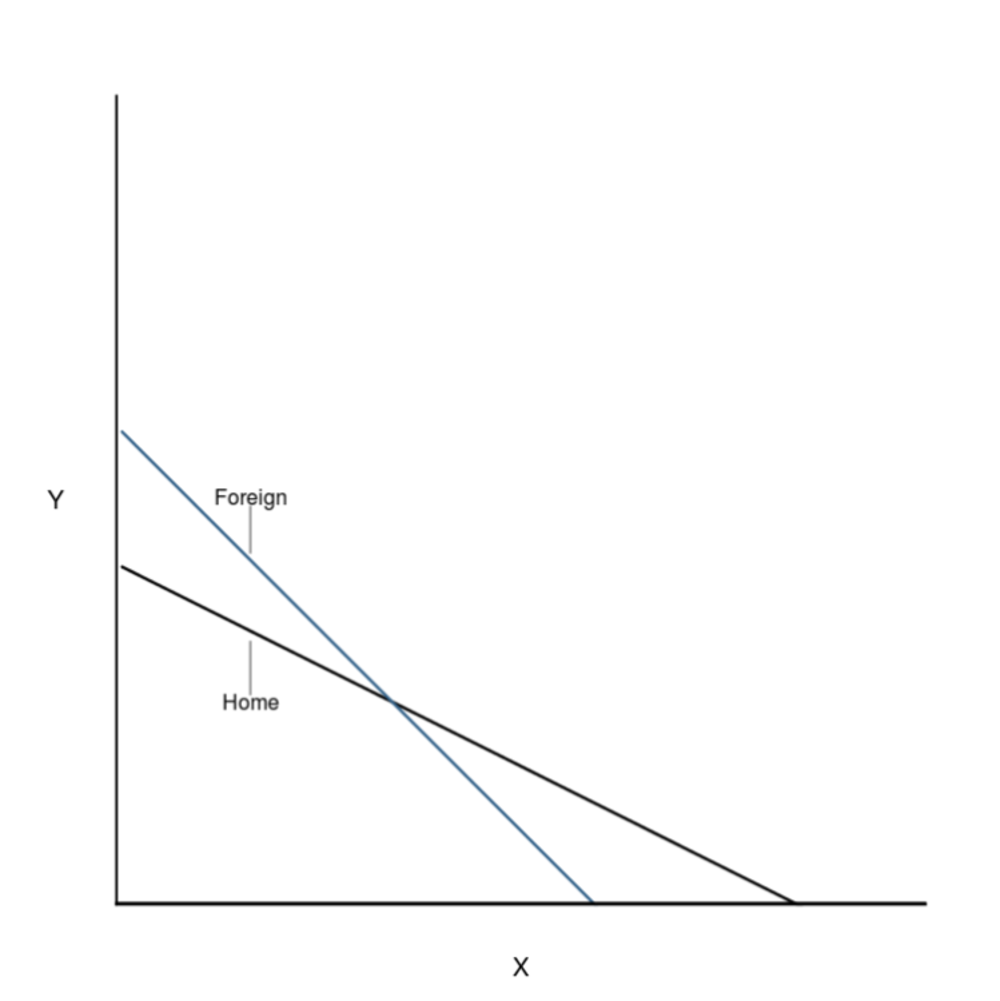
\includegraphics[scale=.8]{ricardo_ppf}
  \end{figure}
\end{frame}
%--------------------------------------

%--------------------------------------
\begin{frame}
  In autarky the PPF acts as a budget constraint for the country.
  \begin{itemize}
    \item In perfectly competitive market the country will produce at highest level of utility within PPF limits
  \end{itemize}  
\end{frame}
%--------------------------------------

%--------------------------------------
\begin{frame}
  Under autarky relative prices under perfect competition are
  \begin{align*}
    p_x=a_x w; p_y=a_yw \Rightarrow p^a =\frac{p_x}{p_y}=\frac{a_x}{a_y}\\
    p_x^*=a_x^* w^*; p_y^*=a_y^*w^* \Rightarrow p^{a*} =\frac{p_x^*}{p_y^*}=\frac{a_x^*}{a_y^*}\\    
  \end{align*}
  Wages are therefore given by
  \begin{align*}
    w &= \frac{p_x}{a_x}=\frac{p_y}{a_y}\\
    w^* &= \frac{p_x^*}{a_x^*}=\frac{p_y^*}{a_y^*}
  \end{align*}
  \textbf{NB -} Wages are equal across sectors.
\end{frame}
%--------------------------------------

%--------------------------------------
\begin{frame}
  In autarky the relative price of good $X$ will be higher in $Home$ than $Foreign$ 
  \begin{align*}
    \frac{p_x}{p_y}>\frac{p_x^*}{p_y^*}
  \end{align*}
  \medskip
  This means that in $Home$ the opportunity costs of $X$ in terms of $Y$ is higher than in $Foreign$.
  \begin{align*}
    \frac{a_x}{a_y}>\frac{a_x^*}{a_y^*}
  \end{align*}
  
\end{frame}
%--------------------------------------

%--------------------------------------
\begin{frame}
  Given  
  \begin{align*}
    \frac{a_x}{a_y} &>\frac{a_x^*}{a_y^*}\\
    \frac{p_x}{p_y} &>\frac{p_x^*}{p_y^*}
  \end{align*}
  suggests that since $Home$ is better at producing $Y$ it should import $X$ from $Foreign$.
  The model therefore predicts two things concerning production and trade patterns;  
  \begin{enumerate}
    \item $Home$ specialises in $Y$ and imports $X$
    \item $Foreign$ specialises in $X$, imports $Y$
  \end{enumerate}  
\end{frame}
%--------------------------------------

%--------------------------------------
\begin{frame}
  Concerning trade patterns each country will export its comparative advantage good
  \begin{itemize}
    \item $Y$ for $Home$ 
    \item $X$ for $Foreign$
  \end{itemize}
  \medskip
  And due to a mutual beneficial exchange, moving from autarky to free trade will imply a price convergence of the two goods
  \begin{align*}
    \frac{p_x}{p_y}=\frac{p_x^*}{p_y^*}
  \end{align*}
\end{frame}
%--------------------------------------

%--------------------------------------
\begin{frame}
  The question that remains is what would be the level of this free trade relative price?\\
  Under free trade three possible equilibria could occur
  \medskip
  \begin{enumerate}
    \item Free trade relative price equals $Home$ autarky relative price
    \item Free trade relative price equals $Foreign$ autarky relative price
    \item Free trade relative price is strictly in between autarky relative prices
  \end{enumerate}
\end{frame}
%--------------------------------------

%--------------------------------------
\begin{frame}
  Scenario 1: Free trade relative price equals $Home$ autarky relative price.
  \begin{align*}
   p^e=p^a=\frac{a_x}{a_y}
  \end{align*}
  \medskip
  \begin{enumerate}
    \item $Home$ keeps producing both goods
    \item $Foreign$ will only produce $X$
  \end{enumerate}
  \medskip
  Only $Foreign$ specialises and will gain, for $Home$ there is no difference between free trade and autarky prices; will not specialise and not gain.
\end{frame}
%--------------------------------------

%--------------------------------------
\begin{frame}
  Scenario 2: Free trade relative price equals $Foreign$ autarky relative price.
  \begin{align*}
   p^e=p^{a*}=\frac{a^*_x}{a^*_y}
  \end{align*}
  This will be similar to the other scenario, in this case
  \medskip
  \begin{enumerate}
    \item $Foreign$ produces both goods
    \item $Home$ produces only $Y$
  \end{enumerate}
  \medskip
  Here $Home$ will gain and $Foreign$ won't.\\   \medskip
  $\Rightarrow$ Scenarios 1 and 2 will lead to a world equilibrium with incomplete specialisation.
\end{frame}
%--------------------------------------

%--------------------------------------
\begin{frame}{World equilibrium with incomplete specialisation}
  \begin{figure}
    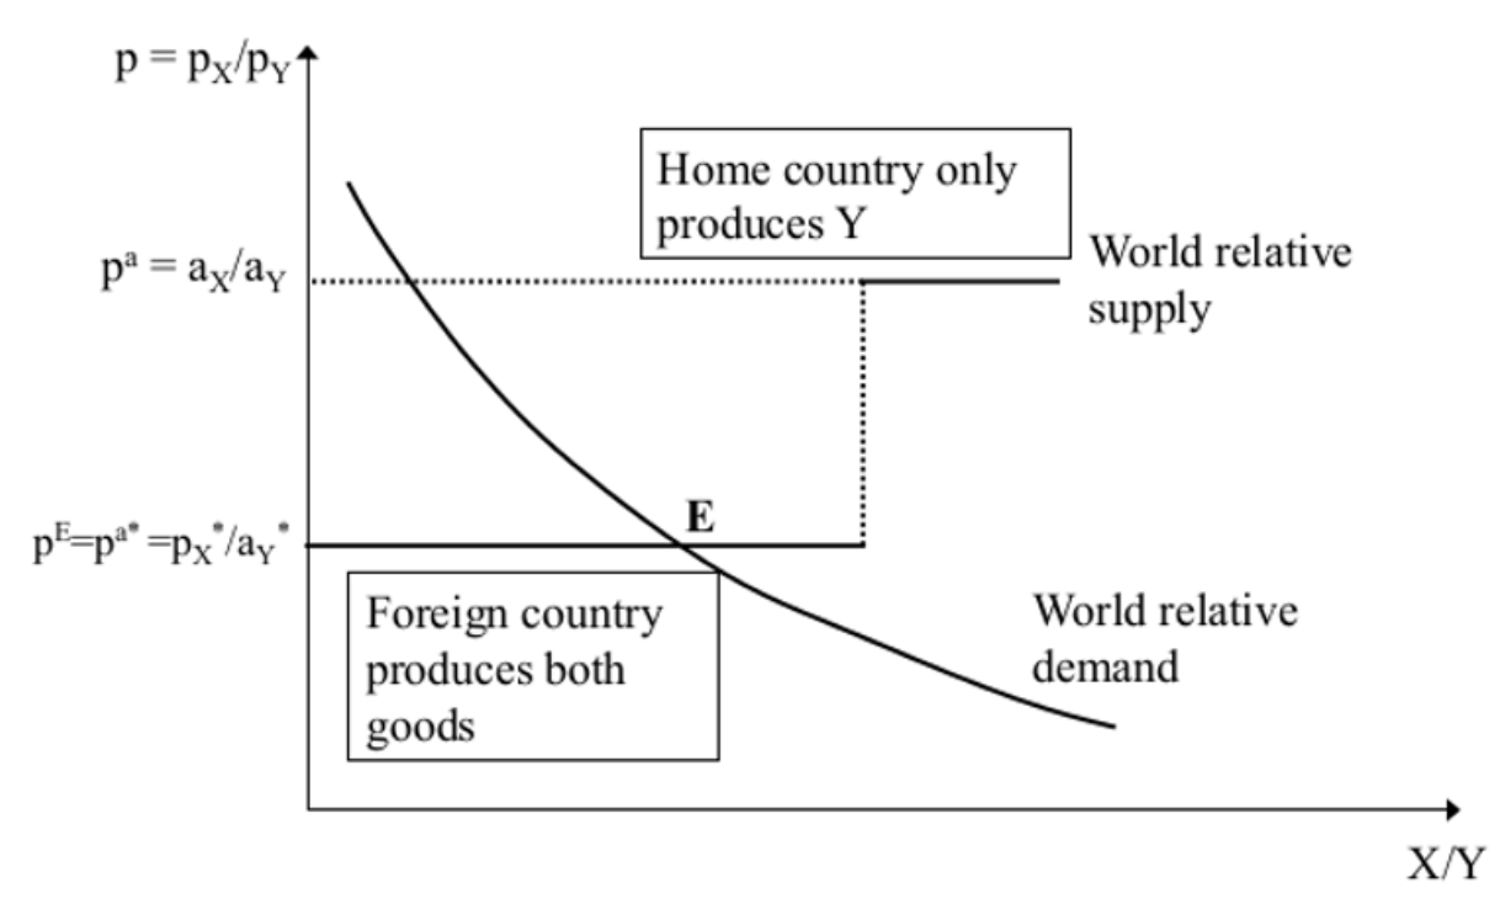
\includegraphics[scale=.8]{ricardo_eq}
  \end{figure}
\end{frame}
%--------------------------------------

%--------------------------------------
\begin{frame}
  Scenario 3: Free trade relative price strictly between autarky relative prices.\\
  This is the equilibrium where we will see full specialisation so
  \begin{enumerate}
    \item $Home$ only produces $Y$
    \item $Foreign$ only produces $X$
  \end{enumerate}
  \medskip
  In this case both countries will gain.   
\end{frame}
%--------------------------------------

%--------------------------------------
\begin{frame}{World equilibrium with complete specialisation}
  \begin{figure}
    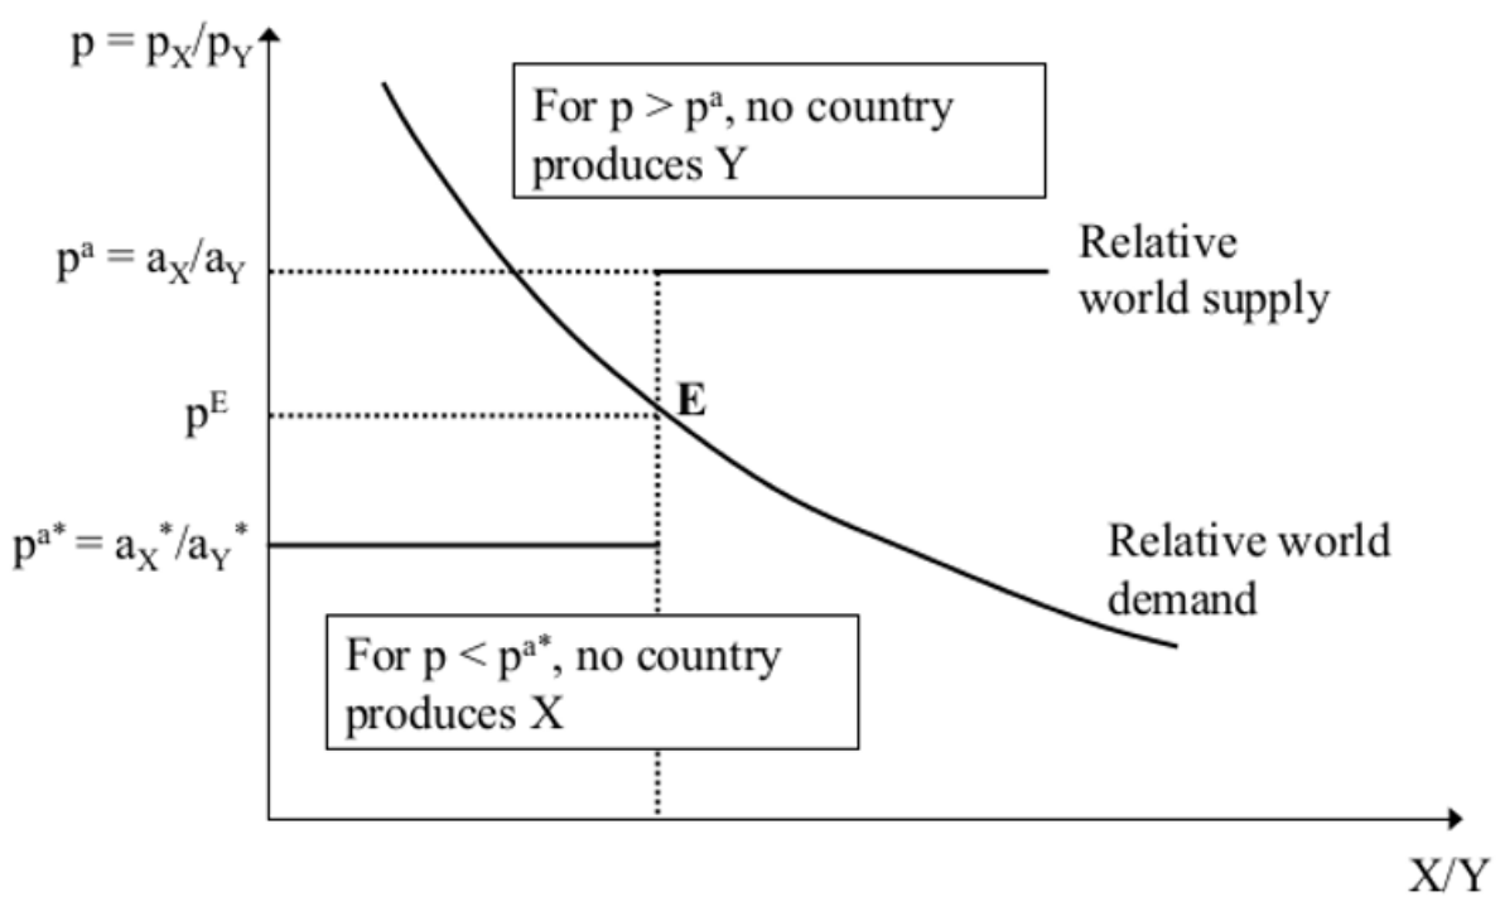
\includegraphics[scale=.8]{ricardo_eq2}
  \end{figure}
\end{frame}
%--------------------------------------

%--------------------------------------
\begin{frame}
  To reiterate, full specialisation will occur if 
  \begin{align*}
    \frac{a_x^*}{a_y^*}<p<\frac{a_x}{a_y}    
  \end{align*}
  \medskip
  Which means that the relative supply of goods will be given by 
  \begin{align*}
    \frac{X}{Y}=\frac{L^*/a_x^*}{L/a_y}
  \end{align*}
\end{frame}
%--------------------------------------

%--------------------------------------
\begin{frame}
  The gains from trade stem from specialisation in the most resource efficient industry and using the generated income to buy desired goods and services
  \begin{itemize}
    \item Again think about Norway using their oil revenue to buy oranges
  \end{itemize}
  Workers can benefit from trade as well since opening up the economy will increase the price of their exported good(s).\\
  \medskip
  \textbf{NB -} In this model we only have one production factor. 
\end{frame}
%--------------------------------------

%--------------------------------------
\begin{frame}
  Trade can be considered as an indirect method of production or acquiring a new technology.
  \medskip
  \begin{itemize}
    \item In absence of trade, country has to allocate resources to produce all the goods it wants to consume
    \item With trade, country can specialise production and trade products for goods it wants to consume
  \end{itemize}
  \medskip
  This means that trade can expand the consumption possibilities beyond the production possibilities. 
\end{frame}
%--------------------------------------

%--------------------------------------
\begin{frame}
  Summarising; opening up to trade $Home$ stops producing $X$
  \begin{itemize}
    \item This will save $a_x$ labour units
  \end{itemize}
  \medskip
  These $a_x$ "additional" labour units are used to produce
  \begin{align*}
    \frac{a_x}{a_y}
  \end{align*}
  more units of $Y$ which are sold to $Foreign$ and the income is used to buy
  \begin{align*}
    \left(\frac{p_y}{p_x}\frac{a_x}{a_y} \right) 
  \end{align*}
  more units of $X$.
\end{frame}
%--------------------------------------

%--------------------------------------
\begin{frame}
 The next diagrams illustrate how production possibilities change as a result of trade. 
 Note that in this case the comparative advantage good of country $A$ will be $X$.
\end{frame}
%--------------------------------------

%--------------------------------------
\begin{frame}{Complete specialisation}
  \begin{figure}
    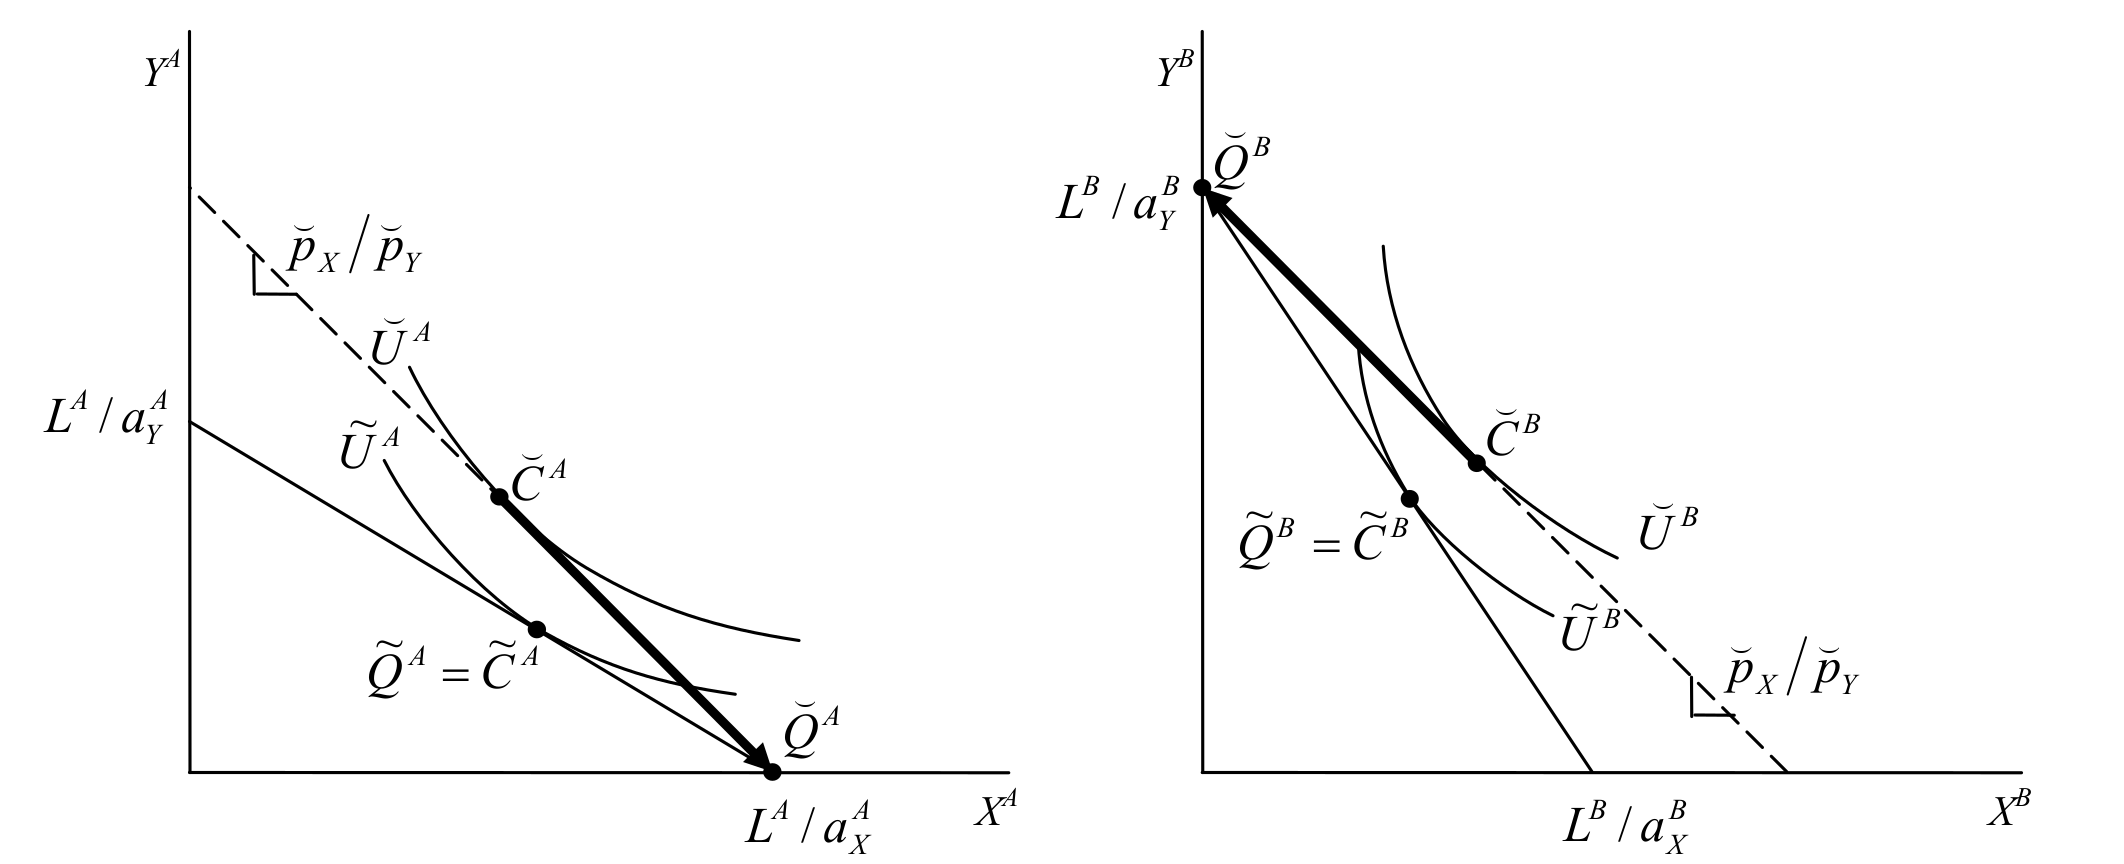
\includegraphics[scale=.6]{deardorff1.png}
  \end{figure}
\end{frame}
%--------------------------------------

%--------------------------------------
\begin{frame}
 Next we consider the case of incomplete specialisation were
 \begin{itemize}
   \item Country $B$'s labour endowment is smaller
   \item Preferences for good $Y$ is larger in both $A$ and $B$
 \end{itemize}
 \medskip
 As a result, the production of country $B$ is too small to meet $A$'s demands, even under $A$'s autarky prices.
\end{frame}
%--------------------------------------

%--------------------------------------
\begin{frame}{Incomplete specialisation}
  \begin{figure}
    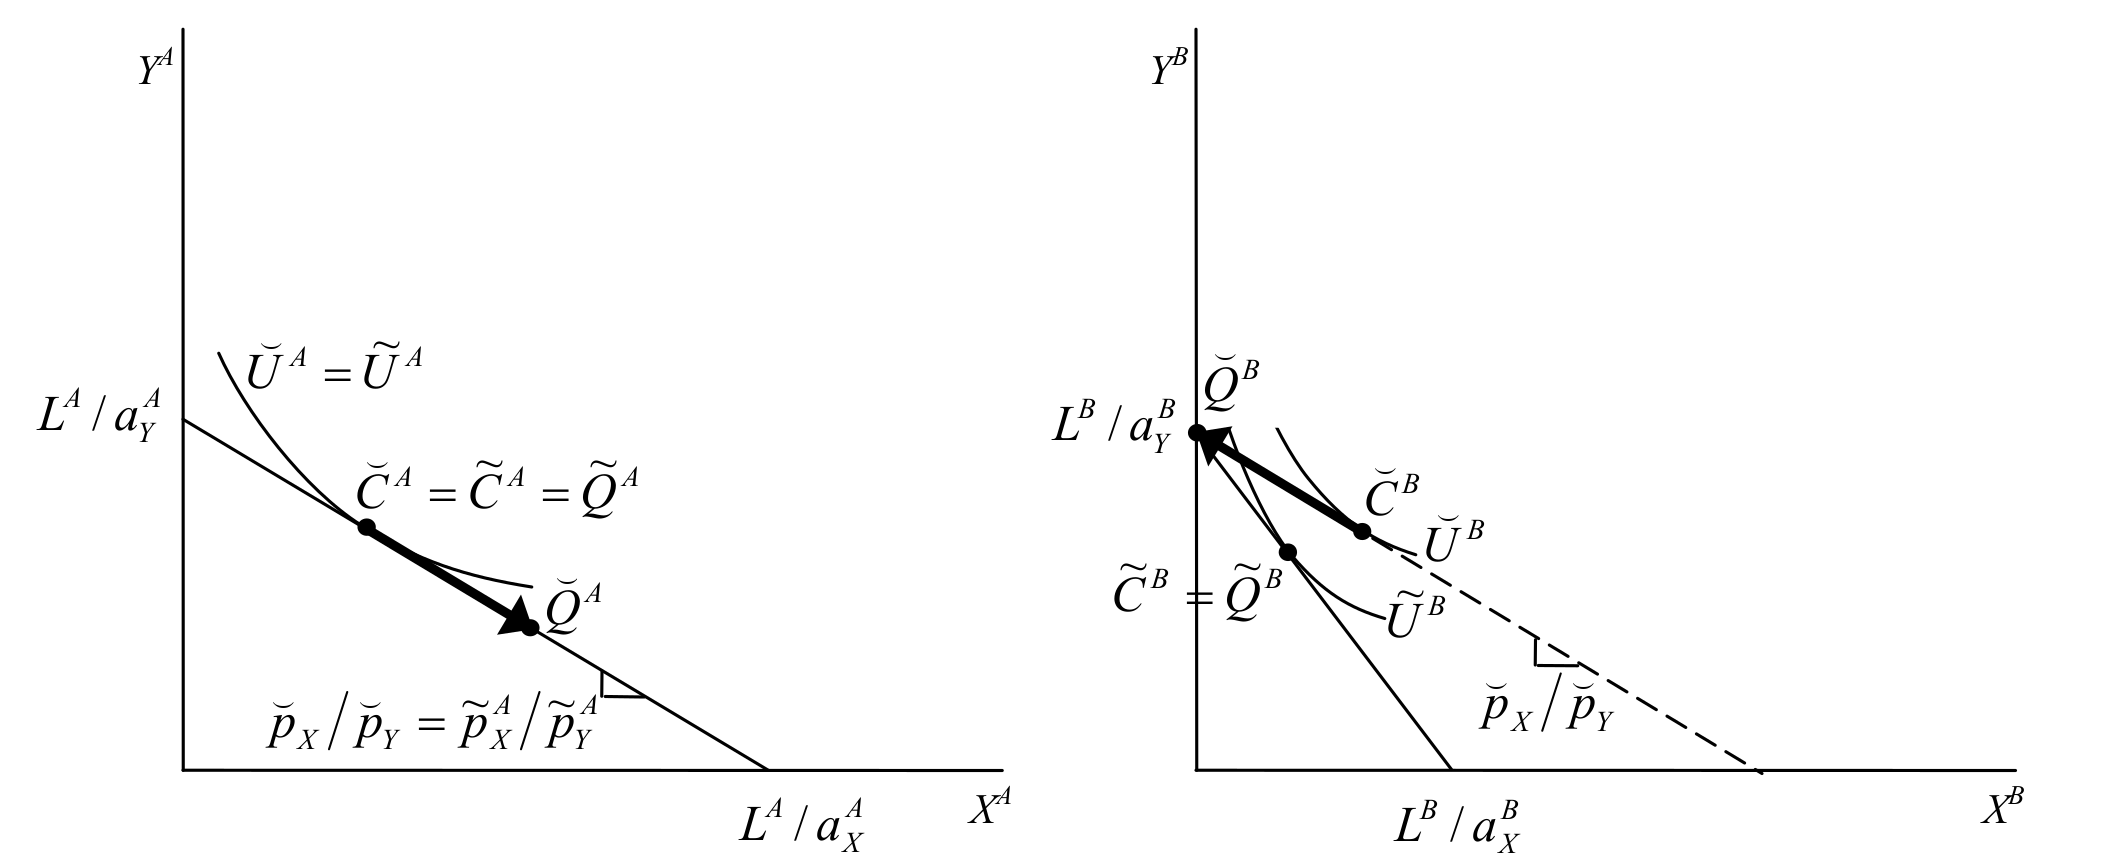
\includegraphics[scale=.6]{deardorff2.png}
  \end{figure}
\end{frame}
%--------------------------------------

%--------------------------------------
\begin{frame}
  Concerning the economic size of trading partners the implications of the model are such that
  \begin{itemize}
    \item The relative price of an export good in a large country will not increase as the partner country is too small to meet demand
    \item Consumption and welfare will be unchanged
  \end{itemize}
  \medskip
  In constrast, for a small country relative prices will change as well as consumption and welfare which will increase.\\
  \medskip
  If both countries are specialised the relative prices of the preferred good will increase and improve the ToT of the exporting country. 
\end{frame}
%--------------------------------------


%--------------------------------------
\begin{frame}
  Workers can benefit from free trade.
  Let's have another look at how their wages are determined.
  Recall that an industry will hire workers until wages equal production value or
  \begin{align*}
    w=p \cdot MPL
  \end{align*}
  \medskip
  This applies to each industry, and since $L$ can move freely between industries, it will move to the highest paying industry until wage equalisation occurs. 
\end{frame}
%--------------------------------------

%--------------------------------------
\begin{frame}
  \begin{align*}
    p_x MPL_x= p_y MPL_y\\
    \frac{p_x}{p_y}=\frac{MPL_y}{MPL_x}
  \end{align*}
  Price ratio $\frac{p_x}{p_y}$ denotes relative price of the numerator good in terms of foregone denominator goods
\end{frame}
%--------------------------------------

%--------------------------------------
\begin{frame}
  From earlier we know that under autarky prices are given by
  \begin{align*}
    p_x^a &= wa_x; p_y^a=wa_y\\
    p_x^{a*} &= w^*a_x^*; p_y^{a*}=w^*a_y^* 
  \end{align*}
  \medskip
  Under full specialisation wages will be determined by the comparative advantage good, i.e. the good that is exported\footnote{Superscripts on prices are dropped here.}
  \begin{align*}
    w &= \frac{p_y}{a_y}\\
    w^* &= \frac{p_x}{a_x^*}
  \end{align*}
  \medskip
  The relative wages are given by
  \begin{align*}
    \frac{w}{w^*} = \frac{p_y}{p_x} \frac{a_x^*}{a_y}
  \end{align*}
\end{frame}
%--------------------------------------

%--------------------------------------
\begin{frame}
  Although trade is determined by comparative advantage, wages are determined by absolute advantage
  \begin{itemize}
    \item In the Ricardian model productivity differences determine wage differences
  \end{itemize}
  \medskip
  Meaning that a country with an absolute advantage in producing a good will enjoy higher wages in that industry after trade.
\end{frame}
%--------------------------------------

%--------------------------------------
\begin{frame}
  The link between wages and productivity has some interesting implications given that it provides countries with an cost advantage in production, specifically
  \medskip
  \begin{enumerate}
    \item High wages cost can be offset by high productivity
    \item Low productivity costs can be offset by low wages
  \end{enumerate}
  \medskip
  This means that technological poor countries can export at competitive prices by having low wages.
  \begin{itemize}
    \item Wages will increase when technology improves
  \end{itemize}
  \medskip
  Therefore, an important prediction of the Ricardian model is that real wages will increase when countries engage in trade.\footnote{Note that this is an implication of the fact that all income accrues to labour.}
\end{frame}
%--------------------------------------

%--------------------------------------
\begin{frame}
  \begin{figure}\centering
    \includegraphics[scale=.3]{koreas}
  \end{figure}
\end{frame}
%--------------------------------------

%--------------------------------------
\begin{frame}
  South Korea, or Republic of Korea
  \begin{itemize}
    \item 11th economy in the world (1.4T USD)
    \item 5th largest exported, 7th largest importer
    \item Highly diversified economy
    \item Reached semi-final of 2002 FIFA World Cop
  \end{itemize}
  \medskip
  In 1960 South Korea's GDP per capita was about 900 USD, lower than most countries in Sub-Sahara Africa.   
\end{frame}
%--------------------------------------

%--------------------------------------
\begin{frame}{Trade relative to GDP in South Korea 1961-2015}
\framesubtitle{source: WDI}
  \begin{figure}
    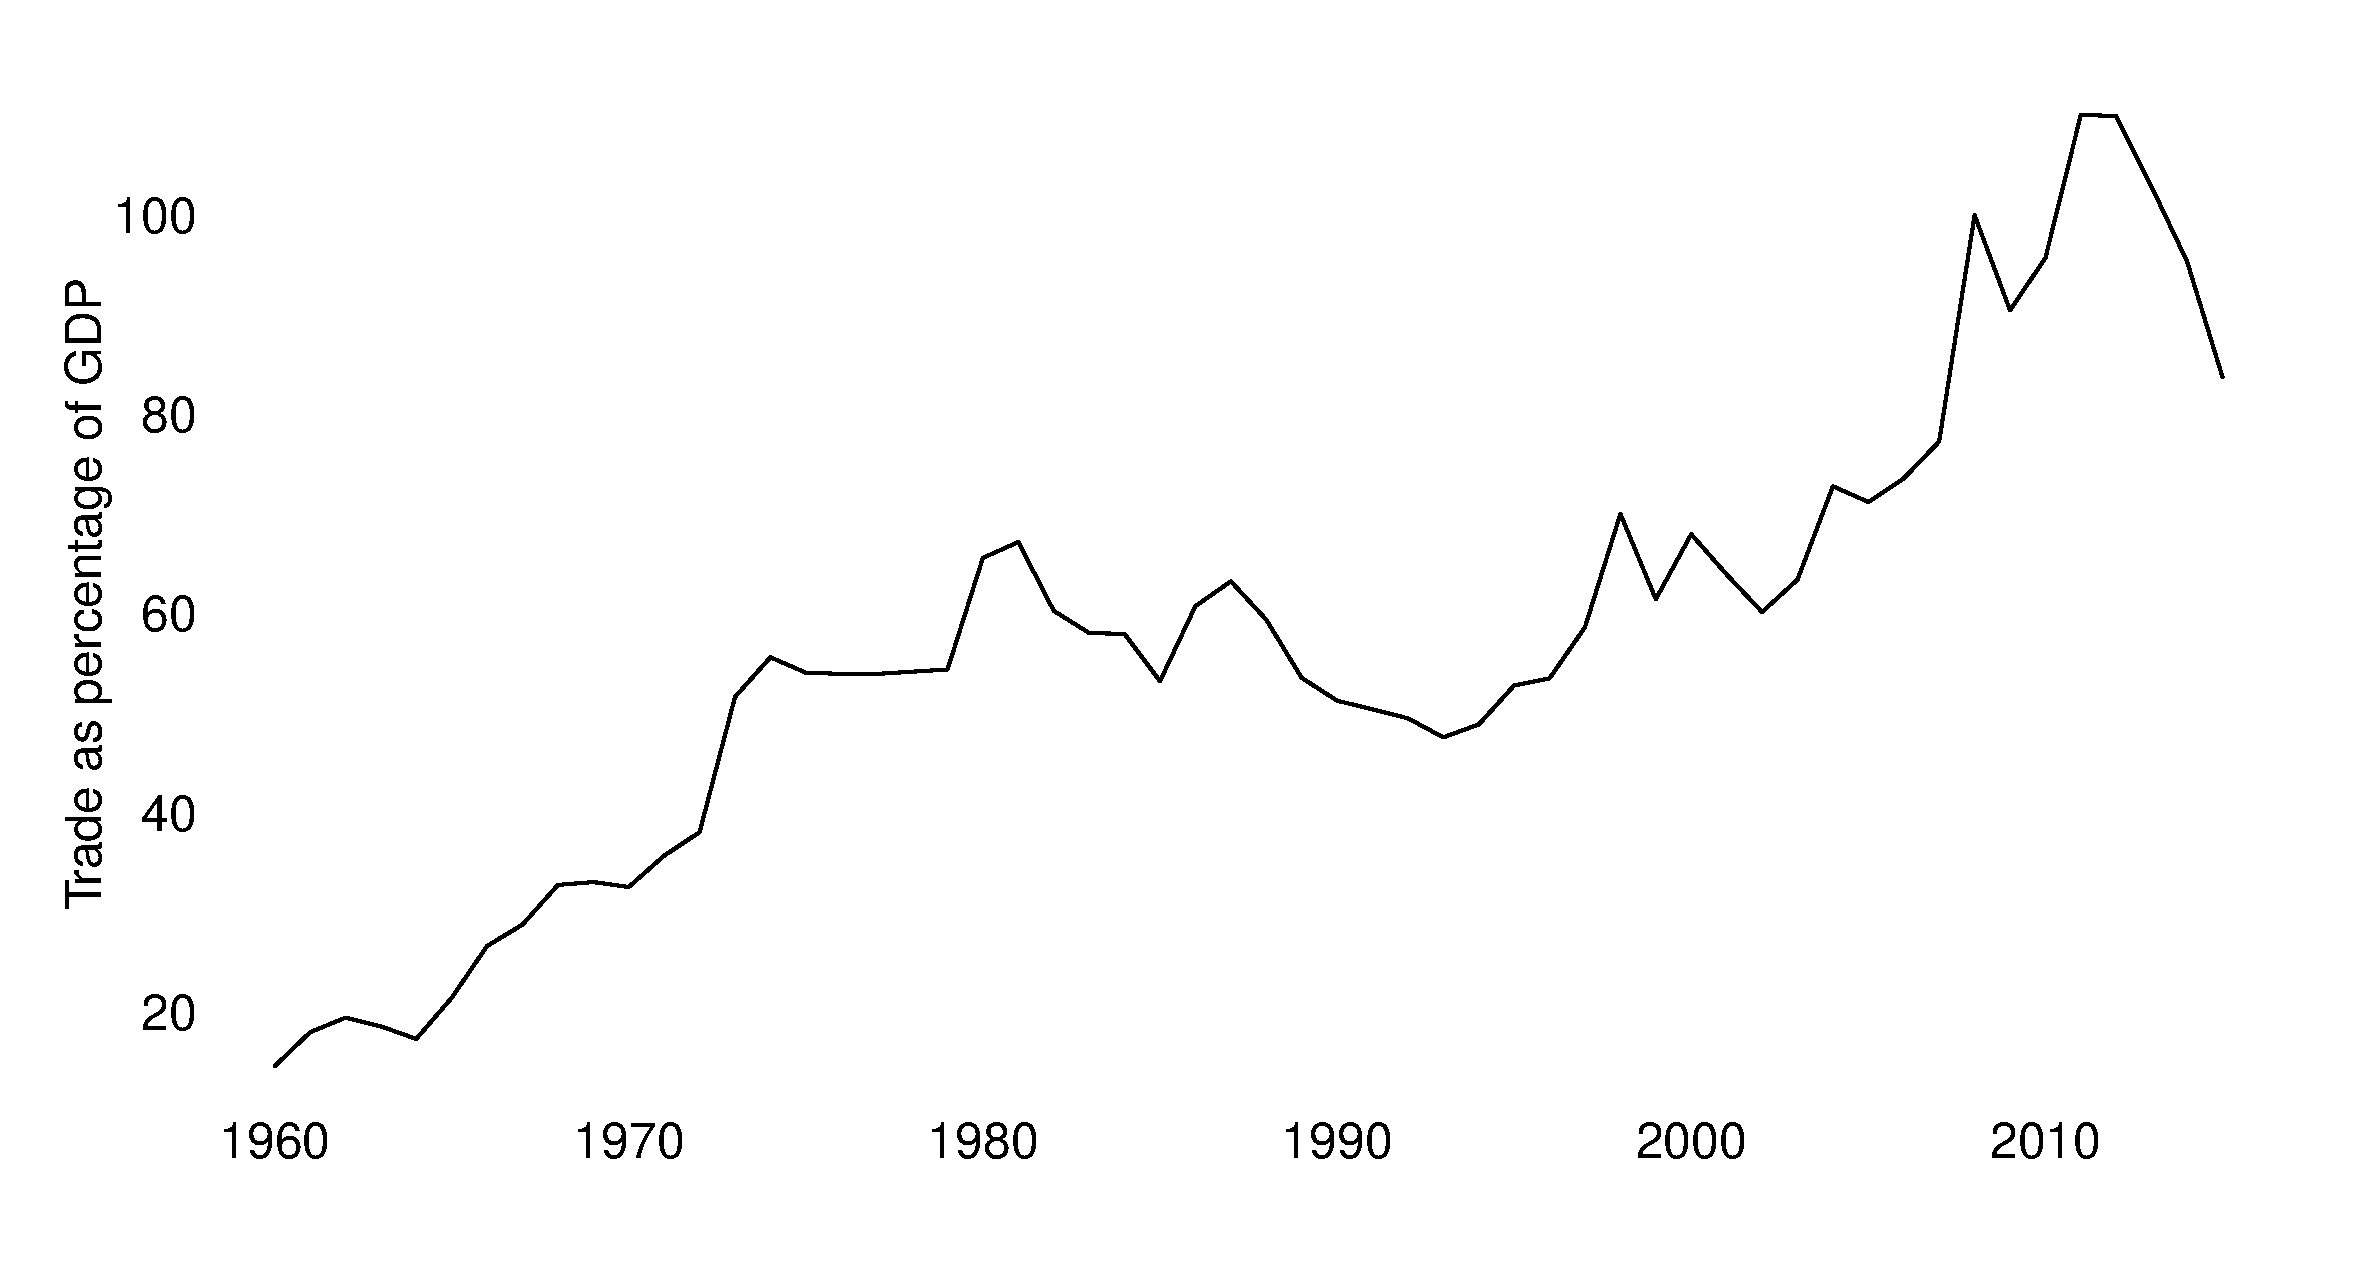
\includegraphics[scale=.3]{korea}
  \end{figure}
\end{frame}
%--------------------------------------

%--------------------------------------
\begin{frame}{Productivity and wages in South Korea 1961-2000}
\framesubtitle{source: UNIDO}
  \begin{figure}
    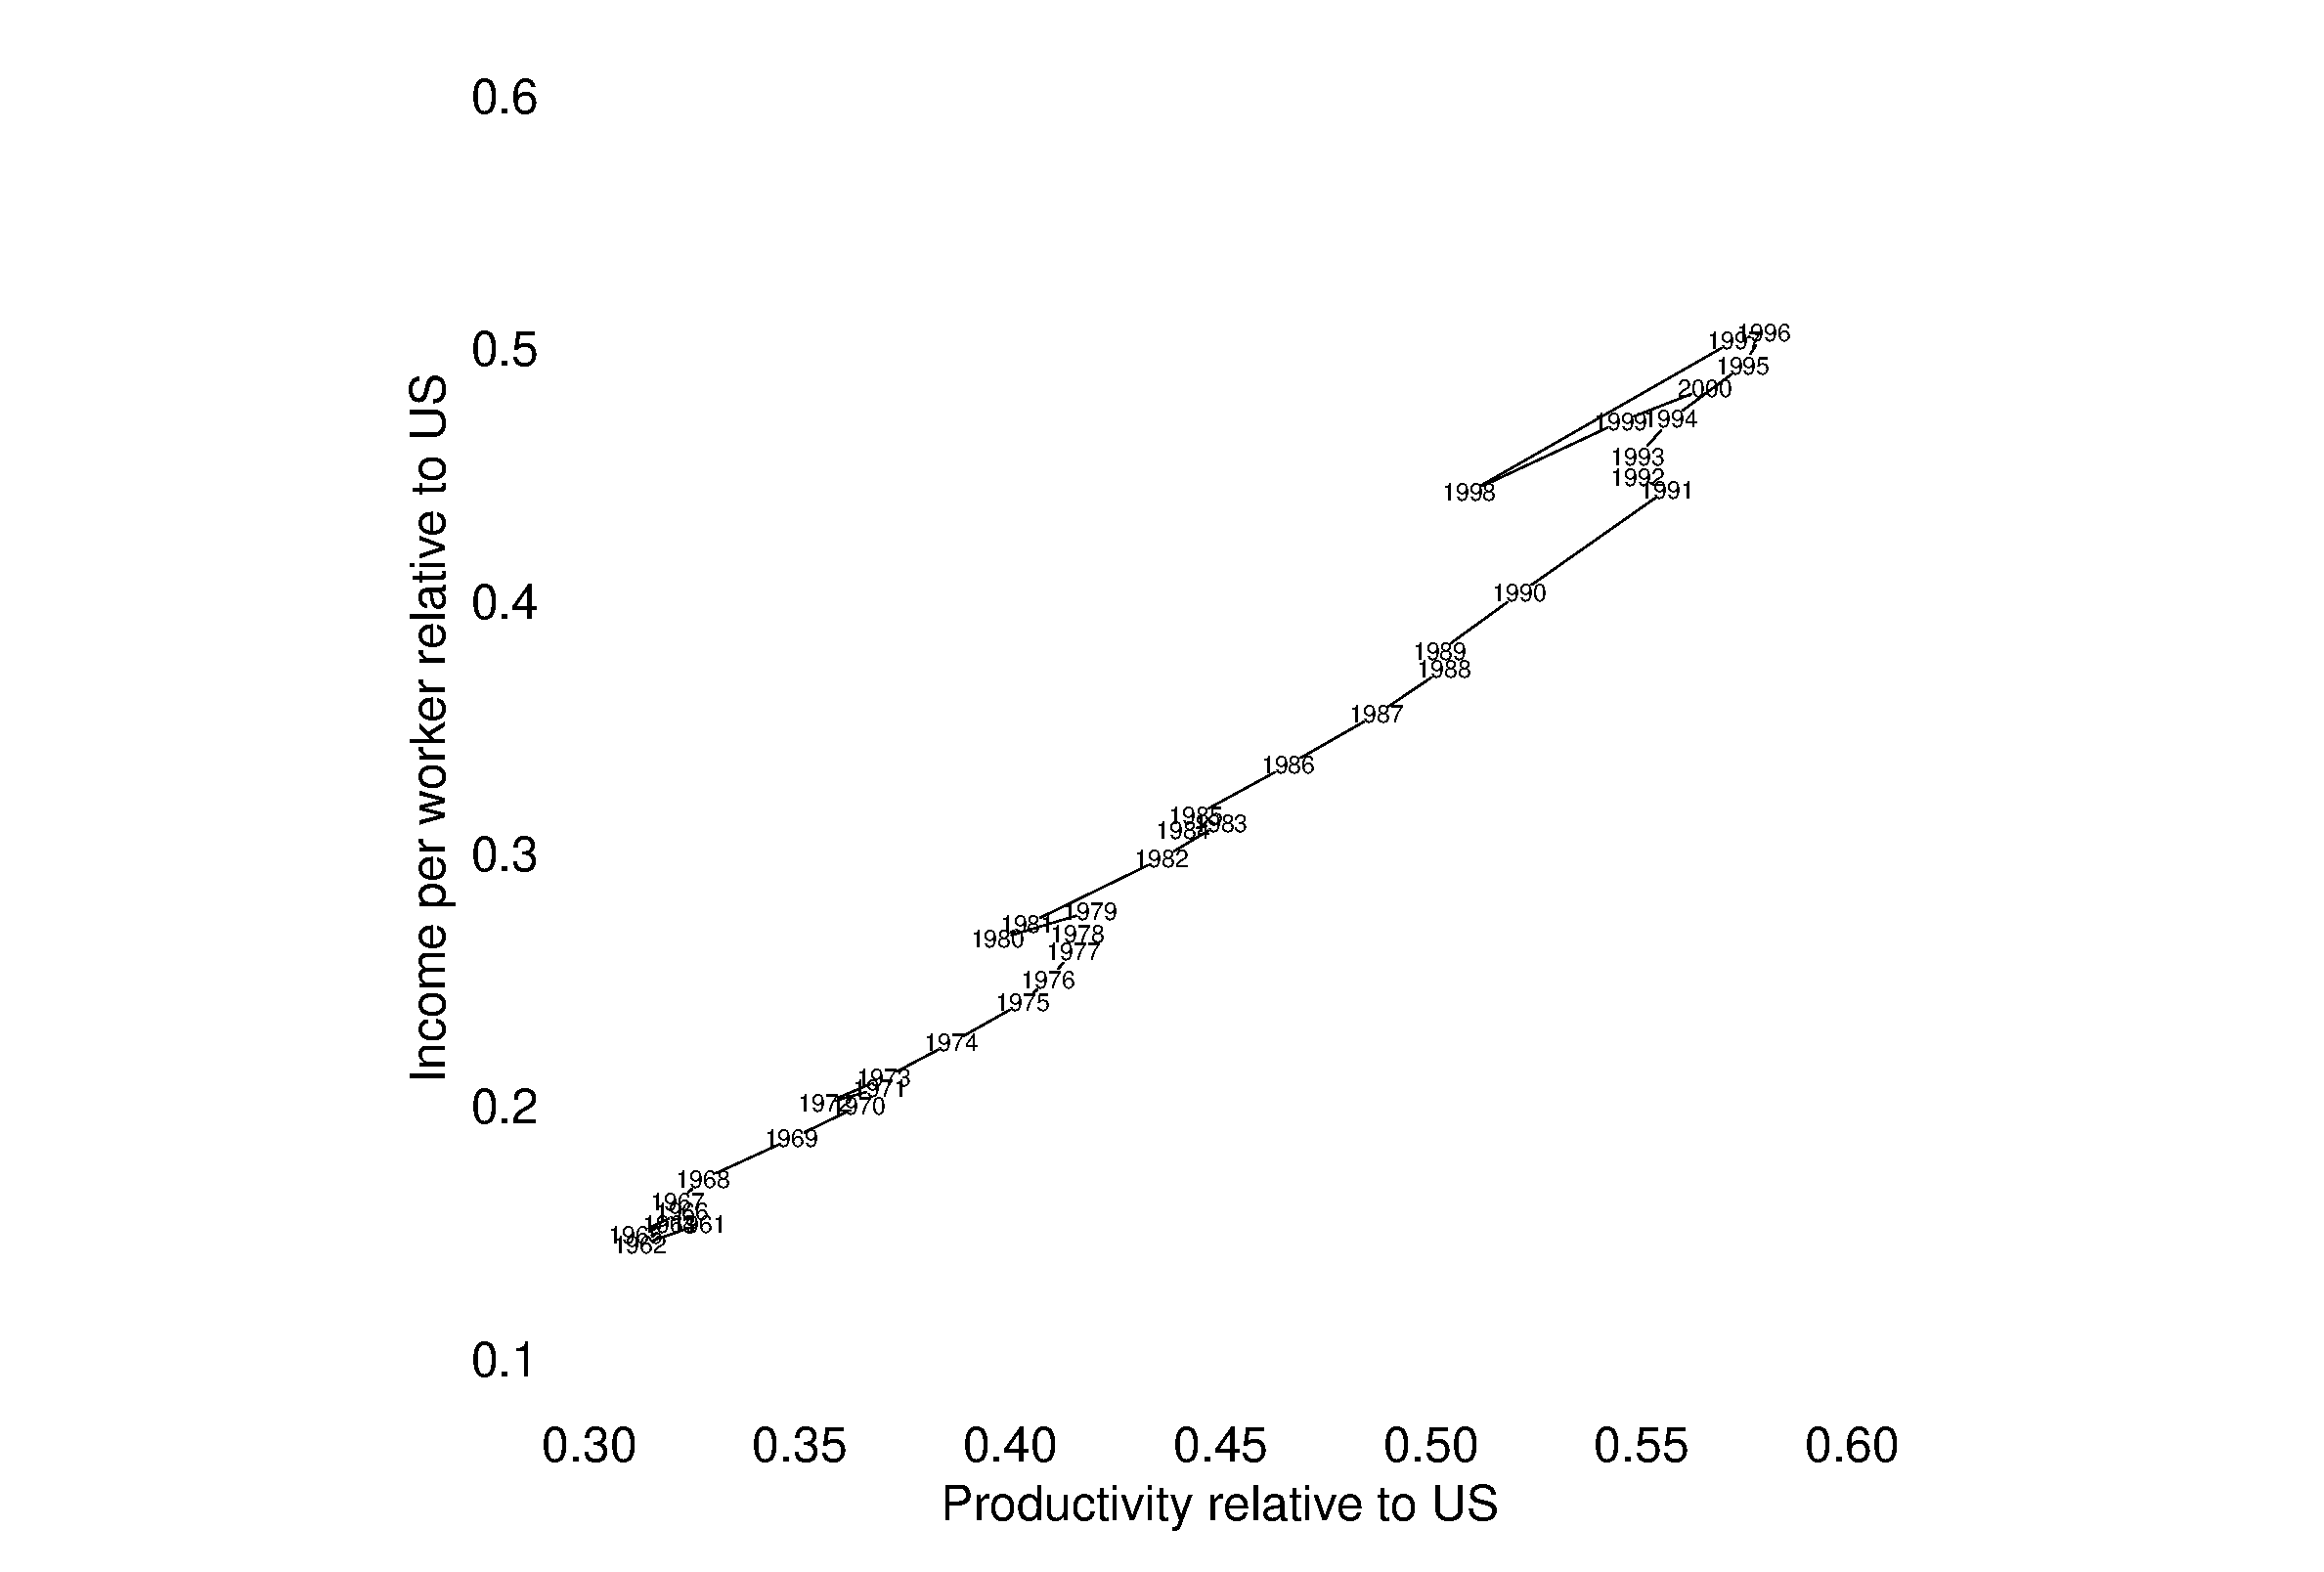
\includegraphics[scale=.25]{korea2}
  \end{figure}  
\end{frame}
%--------------------------------------

%--------------------------------------
\begin{frame}{World productivity and wages in 2000}
\framesubtitle{source: UNIDO}
  \begin{figure}
    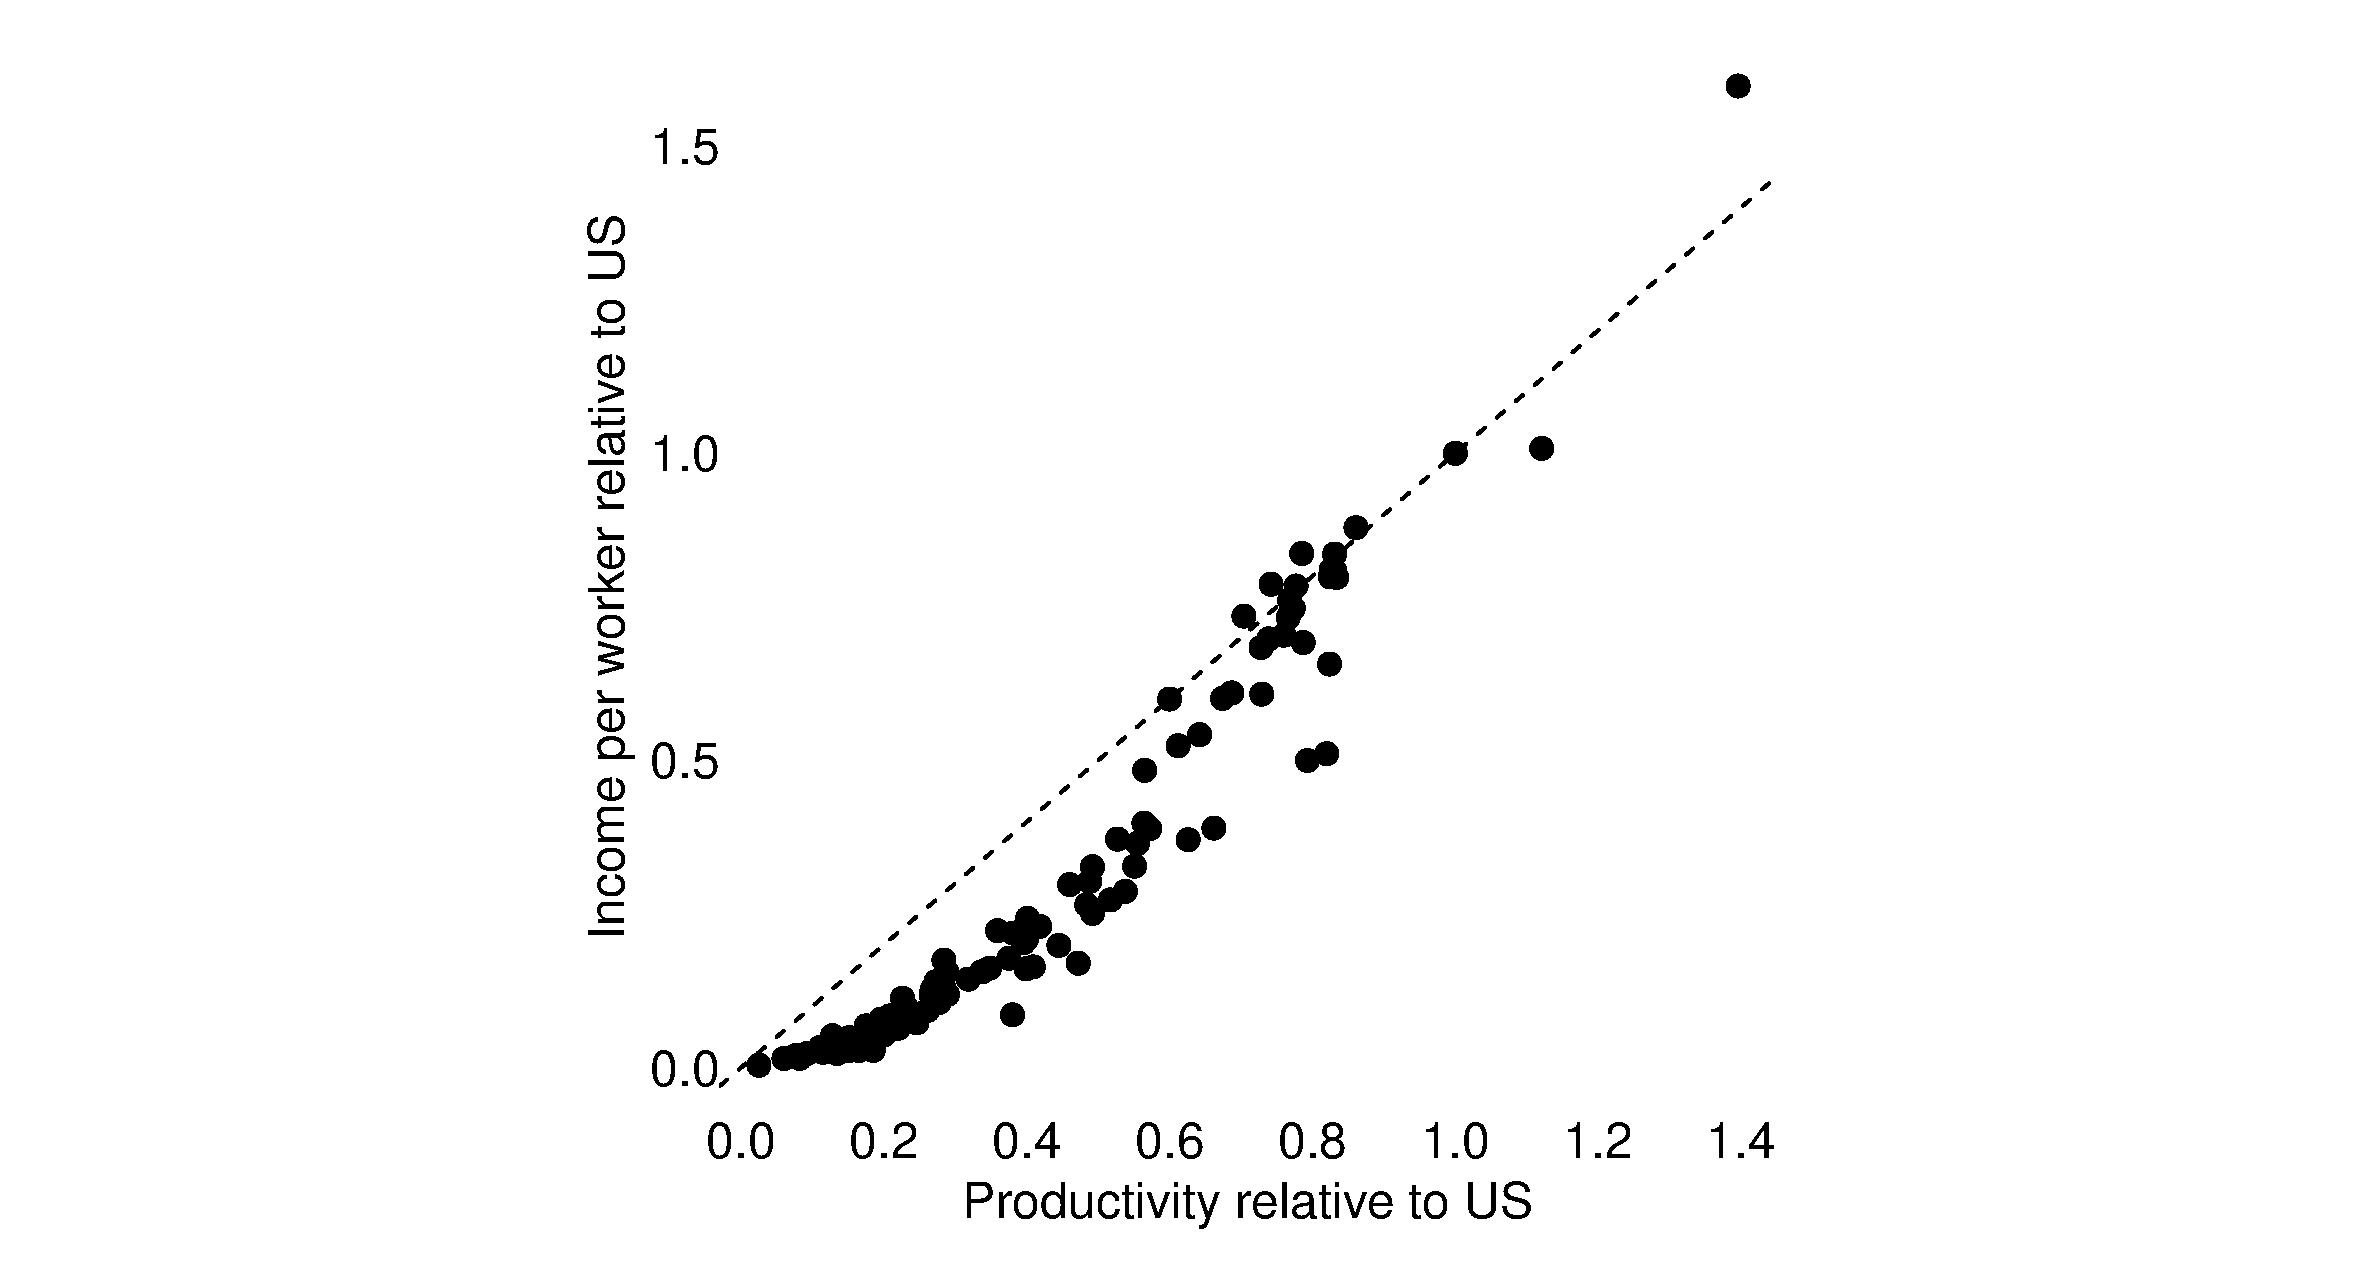
\includegraphics[scale=.3]{global_productivity}
  \end{figure}  
\end{frame}
%--------------------------------------

%--------------------------------------
\begin{frame}{Hourly productivity and labour costs in the EU}
\framesubtitle{source: Eurostat}
  \begin{figure}
    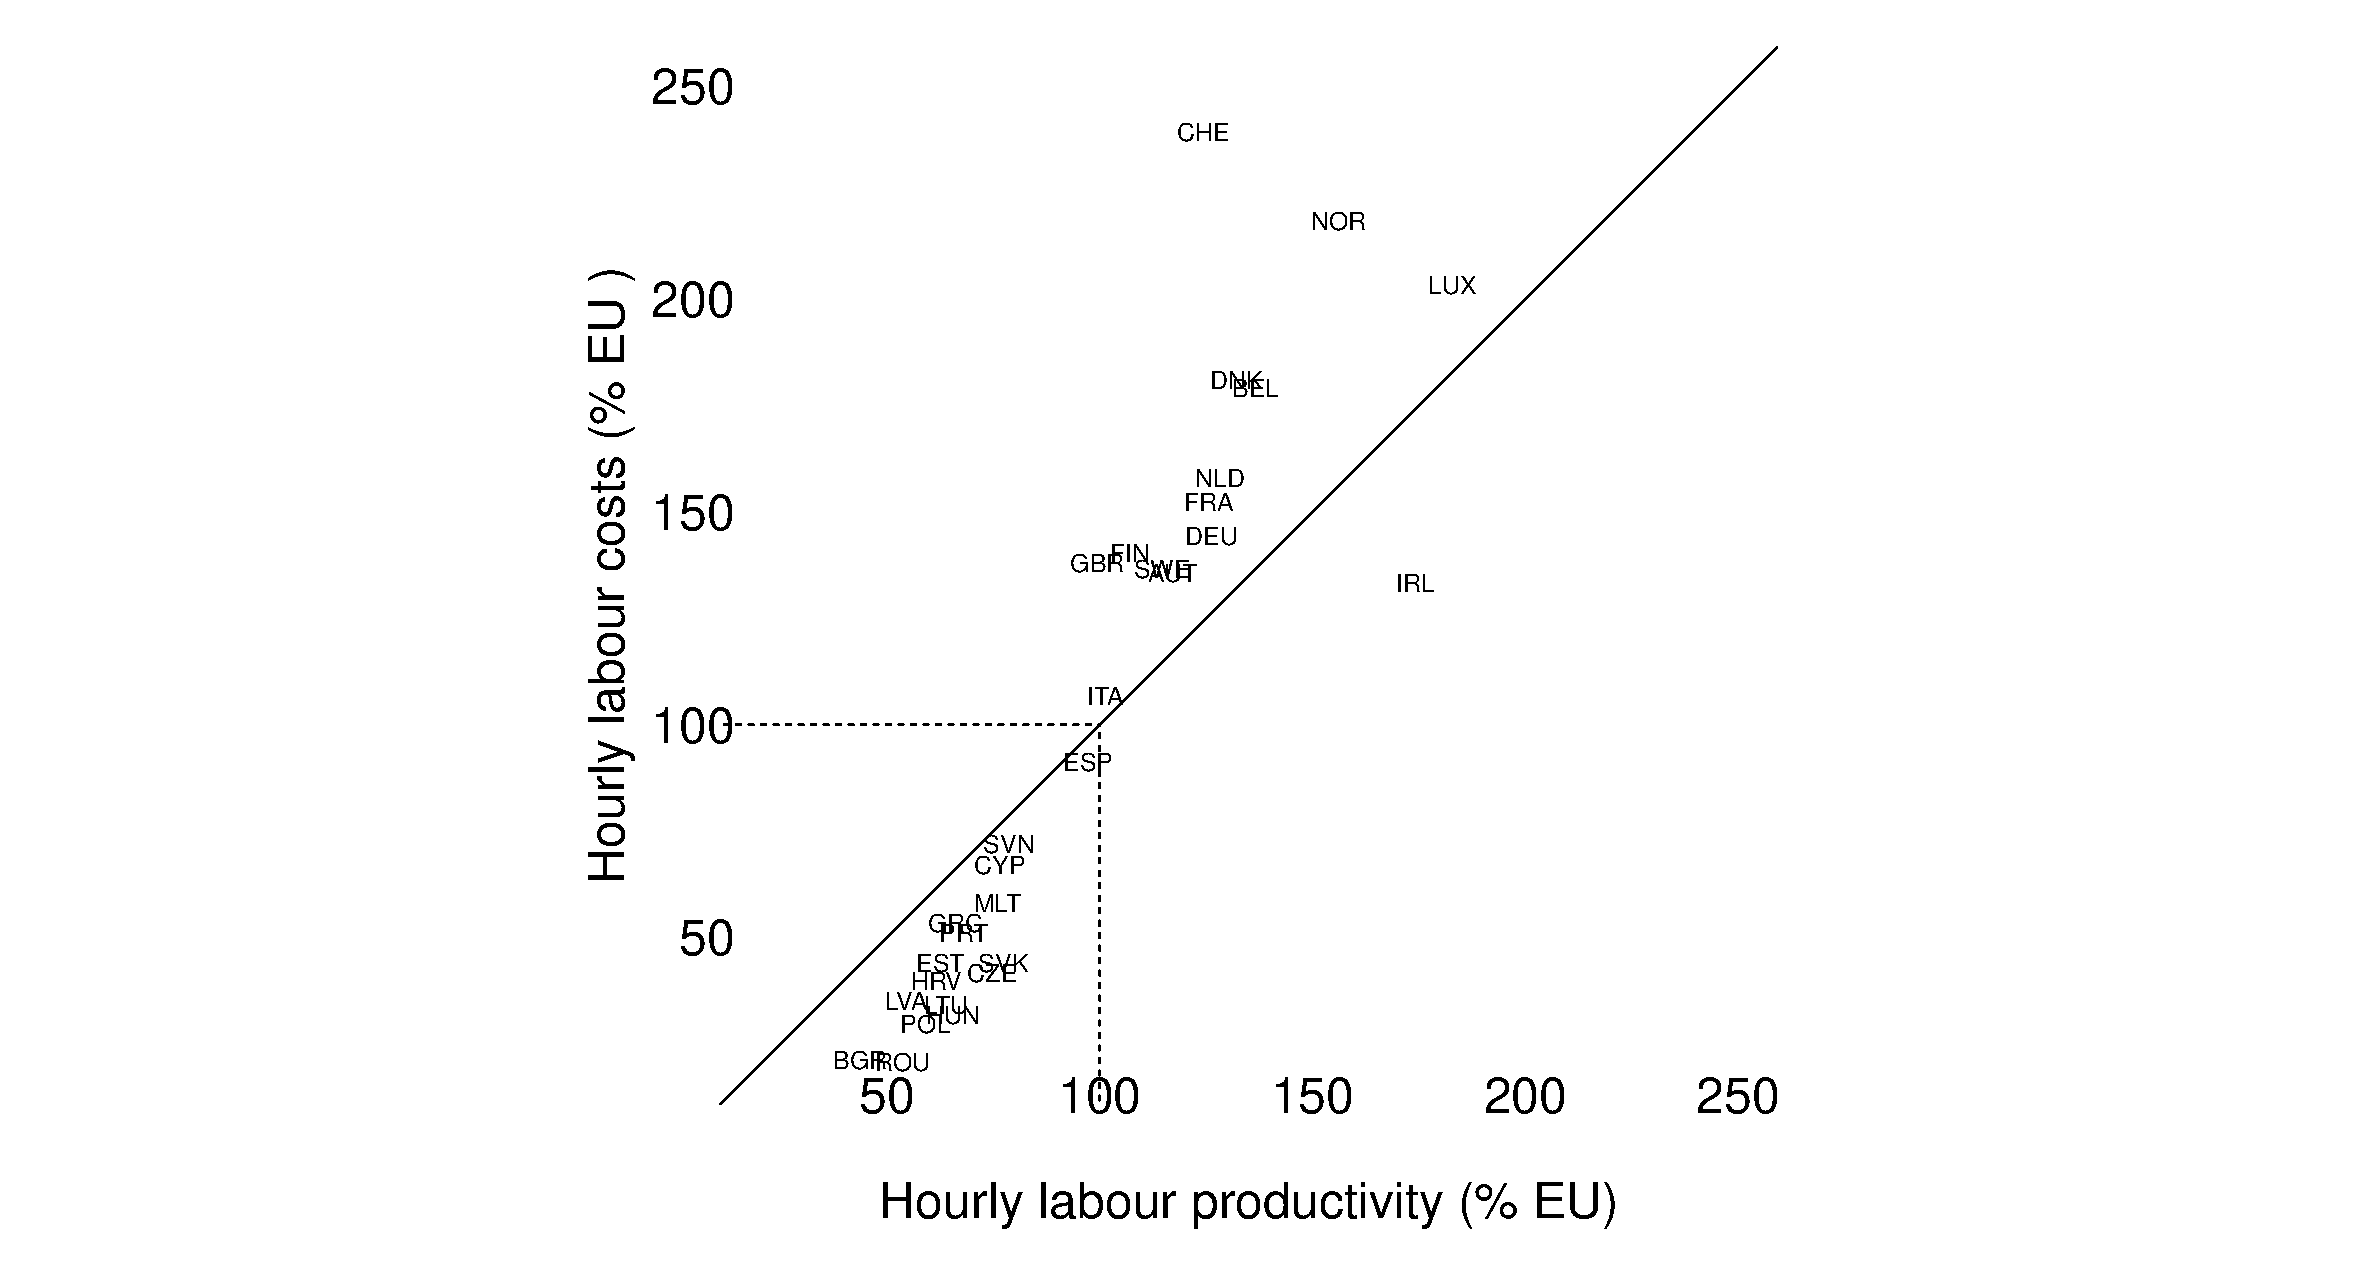
\includegraphics[scale=.3]{wages_productivity}
  \end{figure}  
\end{frame}
%--------------------------------------

%--------------------------------------
\begin{frame}{Bangladesh relative productivity in textiles}
  \begin{figure}
    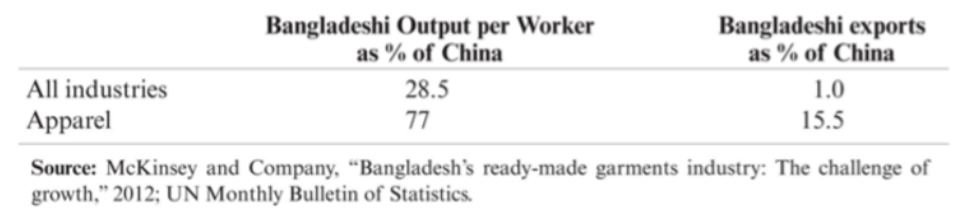
\includegraphics[scale=1.2]{bangladesh2}
  \end{figure}  
\end{frame}
%--------------------------------------

%--------------------------------------
\begin{frame}{US ratio of exports is lowest in least productive sectors in 1951}
  \begin{figure}
    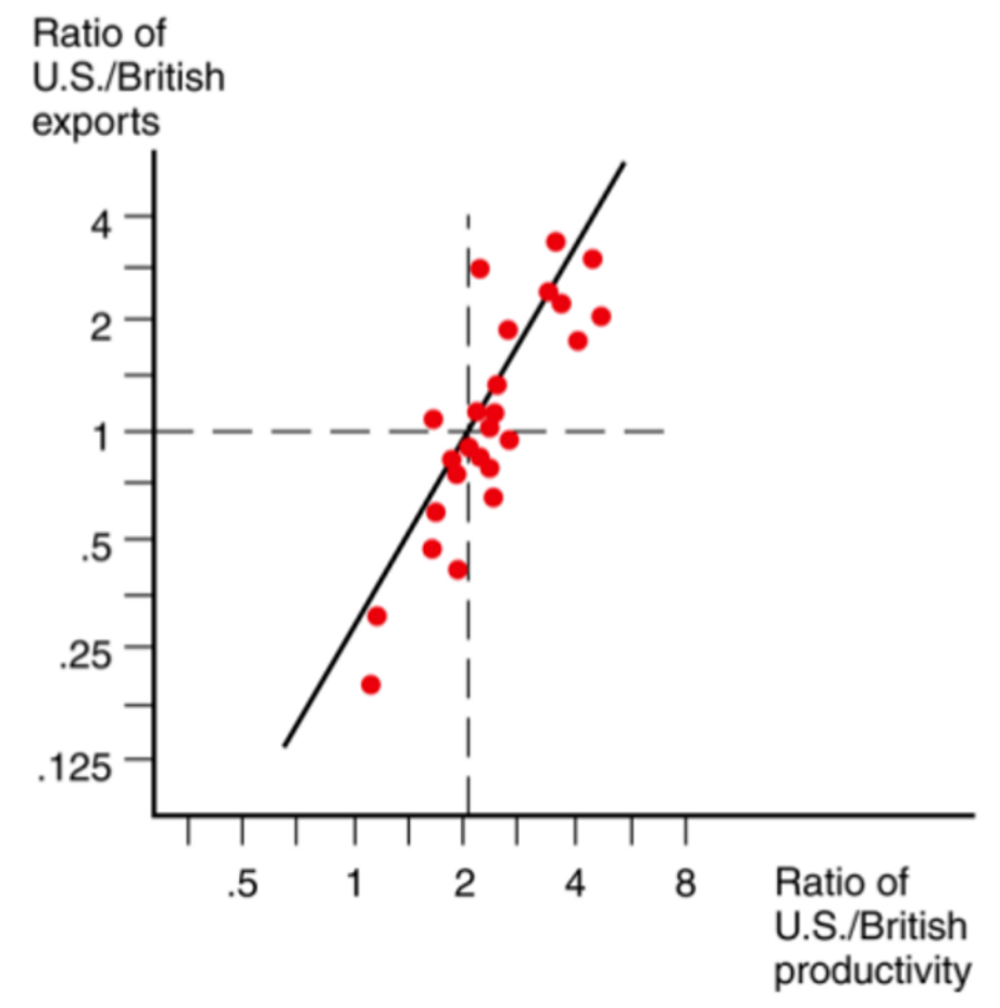
\includegraphics[scale=.8]{us_uk_ratios}
  \end{figure}  
\end{frame}
%--------------------------------------

%--------------------------------------

%--------------------------------------
\begin{frame}
  The Ricardian equilibrium attempt to identify the country that can supply a good at minimum cost. 
  However, the standard model only contains two countries and two goods. 
  In order to apply it to actual world trade we need to add
  \begin{itemize}
    \item More goods
    \item More countries
  \end{itemize}
  \medskip
  Let's run through Ricardo's original example from the beginning, applying what we discussed so far.
\end{frame}
%--------------------------------------

%--------------------------------------
\begin{frame}
\begin{table}{How many workers to make one unit of a good}
  \begin{tabular}{lcc}
    ~ & Cloth (m) & Wine (l) \\
    \hline \\[-1.8ex]\\	
    Portugal  & 90  & 80\\
    England   & 100  & 120\\    
  \end{tabular}
\end{table}  
\medskip
 Let's look at relative wages, Portugal's wage is set equal to 1.
    \begin{table}
    \begin{tabular}{lcc}
      ~ & Cloth (m) & Wine (l) \\
      \hline \\[-1.8ex]\\	
      Portugal  & 90  & 80\\
      England   & 100$w$  & 120$w$\\    
    \end{tabular}
  \end{table}    
\end{frame}
%--------------------------------------

%--------------------------------------
\begin{frame}
  With free trade and perfect competition, prices will be equal in England and Portugal
  \begin{itemize}
    \item It will also be the lowest-cost way of producing each good
  \end{itemize}
  \medskip
  Let's assume that $w$ is larger than the ratio of Portuguese to English workers required for producing cloth ($\frac{90}{100}$).\\
  \medskip
  What will happen to production?  
\end{frame}
%--------------------------------------

%--------------------------------------
\begin{frame}
  Since
  \begin{align*}
    \frac{90}{100} > \frac{80}{120}
  \end{align*}
  \medskip
  both goods will be produced in Portugal, actually leaving English labour unemployed.
  \begin{itemize}
    \item i.e. $w$ must be lower than 90\% of the Portuguese wage
  \end{itemize}
  \medskip
  Similarly, if 
  \begin{align*}
      w<\frac{80}{120}    
  \end{align*}
  \medskip
  both goods will be produced in England, by undercutting the Portuguese wages, leaving the latter unemployed.\\
  \begin{itemize}
    \item So $w$ should be somewhere between $\frac{2}{3}$ and $\frac{9}{10}$
  \end{itemize}
\end{frame}
%--------------------------------------

%--------------------------------------
\begin{frame}
  Let's start with adding an additional good: linen. 
  In this case both Portugal and England require a 100 workers for one unit of linen. 
  We get the following inequality
  \begin{align*}
    \frac{100}{100} > \frac{90}{100} > \frac{80}{120}
  \end{align*}
  \begin{itemize}
    \item England has a stronger comparative advantage in producing linen, compared to cloth, over Portugal. 
  \end{itemize}
  \medskip  
  The ordering of goods in terms of England's relative productivity is called a chain of comparative advantage. 
  Under free trade, relative wage $w$ will break the chain between goods for which England's relative productivity is above or below it's relative wage. 
  \begin{itemize}
    \item For example $w=0.95$ will break it between linen and cloth and wine
  \end{itemize}  
\end{frame}
%--------------------------------------

%--------------------------------------
\begin{frame}
  We can use this chain of comparative advantage to construct a demand curve for English labour as a function of $w$. 
  \begin{itemize}
    \item We assume that both countries spend their money the same way
  \end{itemize}
  \medskip
  Note that for $w>1$ England will price itself out of all goods; for $w=1$ England will be competitive for linen.
  \begin{itemize}
    \item Buyers will be indifferent from the source
  \end{itemize} 
  Any decline $w$ will make England the sole producer of linen, and it will become more competitive at lower wages.  
\end{frame}
%--------------------------------------

%--------------------------------------
\begin{frame}
  \begin{figure}\centering
    
\includegraphics[scale=.7]{ricardo}
  \end{figure}
\end{frame}
%--------------------------------------

%--------------------------------------
\begin{frame}
  This diagram illustrates the intensive and extensive margins of trade
  \begin{itemize}
    \item Intensive margin: exporting more of a given set of goods
    \item Extensive margin: exporting a larger variety of goods
  \end{itemize}
  \medskip
  Decline in $w$ increases England's export demand at the intensive margin until it reaches a threshold where it expands at the extensive margin.   
\end{frame}
%--------------------------------------

%--------------------------------------
\begin{frame}
  More general, the Ricardian model can be extended by ranking all the goods based on productivity
  \begin{align*}
    \frac{a_1^*}{a_1}<\frac{a_2^*}{a_2}<...<\frac{a_n^*}{a_n}
  \end{align*}
  \medskip
  For this series locate $\frac{w}{w^*}$ and home will export goods
  \begin{align*}
    \frac{a_i^*}{a_i}>\frac{w}{w^*}
  \end{align*}
  \medskip
  Wage disadvantage is compensated by advantage in productivity
\end{frame}
%--------------------------------------

%--------------------------------------
\begin{frame}
  It is straightforward to expand the model to include more countries
  \begin{itemize}
    \item Although not more countries and more goods at the same time
  \end{itemize}
  \medskip
  Let's add France with the following labour requirements
  \begin{itemize}
    \item 60 in wine
    \item 120 in cloth    
  \end{itemize}
  \medskip
  We can use the chain to produce
  \begin{align*}
    \frac{120}{100} > \frac{80}{90} > \frac{60}{120}
  \end{align*}
  \medskip
  Here England will produce cloth and France will produce wine.   
\end{frame}
%--------------------------------------

%--------------------------------------
\begin{frame}
  Although the economic ideas of Ricardo are 200 years old, they provide some powerful arguments in favour of free trade. 
  Nonetheless, there are still some popular misconceptions concerning trade, for instance
  
  \begin{enumerate}
    \item Trade only helps the more productive countries
    \begin{itemize}
      \item Specialisation allows unproductive countries by using resources more efficiently
    \end{itemize}
    \medskip
    \item Industrialised countries are hurt by low wage countries
    \begin{itemize}
      \item Consumers in industrialised countries benefit from cheaper products
      \item Although trade can bring disadvantages for certain groups
    \end{itemize}
    \medskip
    \item Trade hurts developing countries as exports require low wages
    \begin{itemize}
      \item Consider alternative in absence of trade
    \end{itemize}
  \end{enumerate}
\end{frame}
%--------------------------------------

%--------------------------------------
\begin{frame}
  Although the Ricardian model can help understand trade patterns, the predicted specialisation rarely happens
  \medskip
  \begin{enumerate}
    \item Transportation costs reduce/hamper trade
    \item Multiple production factors which reduce specialisation tendency
    \item Protectionism
  \end{enumerate}
\end{frame}
%--------------------------------------

%--------------------------------------
\begin{frame}
  Concerning transportation costs, and briefly going back to the gravity model; the Ricardian model can be adjusted to account for transport costs.\\
  Let $\tau$ be proportional transport cost, then good $i$ is not traded when
  \begin{align*}
    wa_i < w^*a_i^*<wa_i(1+\tau)
  \end{align*}
\end{frame}
%--------------------------------------


%------------------------------------------------------------------------------
\end{document}
